\chapter{تمايز الخلايا: الخلية العضلية الهيكلية}\label{ch:b2:cell-differentiation}

ليفة من عضلة فخذك خلية واحدة طولها ثلاثون
سنتيمترًا، ولها مئات النوى، محشوة من طرف إلى طرف
بقضبان قابضة منتظمة انتظامًا يجعلها مخططة تحت
المجهر. وقد بدأت عنقودًا من خلايا عادية المظهر
زحفت من قُطَيعة، وتكاثرت، وكفّت عن الانقسام، واصطفت،
واندمجت، وأشعلت عدة مئات من المورّثات لم تستعملها
من قبل. ولكل خلية في الجسم المورثوم نفسه؛ \omterm{def:b2:cell-differentiation:myogenesis}{والليفة العضلية}
هي ما يفعله ذلك المورثوم حين يُشعل \omterm{prop:b2:cell-differentiation:transcriptional}{عامل استنساخ} واحد
بعينه. يتخذ هذا الفصل الخلية العضلية الهيكلية مثالًا
محلولًا على \emph{\omterm{def:b2:cell-differentiation:differentiation}{التمايز}} --- أي كيف تكتسب الخلية
هويةً متخصصة وتحفظها --- والخلية العضلية مثال جيد
لأن المفتاح الرئيس معروف، والخطوات يمكن مراقبتها في
طبق، والخلية النهائية آلة أجزاؤها مرئية.

\section{ما التمايز}

\begin{definition}[التمايز والتحدد والقدرة]\label{def:b2:cell-differentiation:differentiation}
\index{تمايز}\index{تحدد}\index{خلية جذعية}\index{قدرة}
تكون الخلية \emph{متمايزة} حين تعبّر عن النميط الثابت
من المورّثات --- ومن ثم عن البروتينات والشكل والوظيفة --- الذي
لصنف خلوي واحد. وتكون \emph{متحددة} (أو ملتزمة) حين يثبت مصيرها
مع أن تمايزها لم يبدأ بعد: \omterm{def:b2:cell-differentiation:myogenesis}{فالأرومة العضلية}
تبدو كأرومة ليفية لكنها لن تصنع إلا عضلًا. و\emph{القدرة}
هي مدى الأصناف التي لا تزال الخلية تستطيع إعطاءها:
\emph{\omterm{prop:b2:asexual-reproduction:tissueculture}{كلية القدرة}} (اللاقحة والفلجات الأولى، وهي تصنع كل شيء بما فيه
\omterm{def:b2:mammal-reproduction:placenta}{المشيمة})، و\emph{متعددة القدرة} (\omterm{def:b2:mammal-reproduction:implantation}{الكتلة الخلوية الداخلية}، وهي تصنع
كل نسيج في الجسم)، و\emph{متعددة القدرة المحدودة} (خلية جذعية
من الدم أو من العضل، وهي تصنع أصناف نسيج واحد)،
و\emph{أحادية القدرة}. و\emph{الخلية الجذعية} خلية تنقسم فتعطي
بنتًا مثلها وأخرى تمضي إلى التمايز،
وهذا يبقي المخزون ويمون النسيج في آن. والتمايز
في معظم الحالات ليس فقدًا لمورّثات بل اختيارًا بينها: فمورثوم
نواة عضلية كامل.
\end{definition}
\begin{proof}[شواهد]
زرع غوردون (1962) نواة خلية معوية متمايزة من
شرغوف في بيضة ضفدع أُتلفت نواتها؛
فنما جزء من البيوض ضفادع سوية
خصيبة. فالنواة المتمايزة لم تفقد شيئًا من
المورّثات اللازمة لصنع حيوان كامل؛ وإنما أعاد سيتوبلازم البيضة
ضبطها. والعملية نفسها بنواة خلية ثديية في بيضة نعجة
أعطت دوللي (1996)، وبيّنت إعادة برمجة أرومة ليفية جلدية إلى
\omterm{def:b2:cell-differentiation:differentiation}{خلية جذعية} متعددة القدرة بأربعة \omterm{prop:b2:cell-differentiation:transcriptional}{عوامل استنساخ} (ياماناكا،
2006) أن إعادة الضبط تتم بحفنة من البروتينات.
\end{proof}

\begin{proposition}[التمايز أمر استنساخي]\label{prop:b2:cell-differentiation:transcriptional}
\index{عامل استنساخ}\index{منظّم رئيس}
الفرق بين صنفين خلويين يكمن في أي المورّثات
تُستنسخ. فبضعة \emph{\omterm{prop:b2:cell-differentiation:transcriptional}{عوامل استنساخ}}، يُعبَّر عنها
استجابةً لإشارات الاستحثاث في
\cref{ch:b2:vertebrate-development}، ترتبط بالمناطق التنظيمية
لمئات المورّثات الهدف وتشعلها، بينما تُطفأ مورّثات
المصائر الأخرى؛ ولأن عاملًا كهذا ينشّط عادةً
مورّثته هو، تصون الحالةُ نفسَها متى دخلتها الخلية.
وفي بعض الأنسجة يكون عامل واحد \emph{منظّمًا رئيسًا}
كافيًا لفرض المصير على خلية من صنف آخر: وهو \omterm{def:b2:cell-differentiation:myogenesis}{MyoD}
للعضل الهيكلي، وPax6 للعين، وSox9 للغضروف. وتزداد الحالة
ثباتًا بتغيرات في الصبغين --- مثيلة
DNA، وتعديل الهستونات --- تبقي المورّثات المسكتة
مسكتة عبر الانقسامات (وهو \emph{علم التخلّق} في مجلد السنة
الثالثة). فالخلية المتمايزة تتذكر إذن ما هي
دون أي تغير في تسلسل دناها، والذاكرة مكتوبة
في نميط العوامل والصبغين، لا في المورّثات.
\end{proposition}

\section{صنع ليفة عضلية}

\begin{definition}[تكوّن العضل]\label{def:b2:cell-differentiation:myogenesis}
\index{أرومة عضلية}\index{أنبوب عضلي}\index{ليفة عضلية}\index{MyoD}
في الجنين، تُستحث خلايا الأديم الجلدي العضلي من القُطَيعة
بإشارات من \omterm{prop:b2:vertebrate-development:neurulation}{الأنبوب العصبي} \omterm{prop:b2:vertebrate-development:gastrulation}{والحبل الظهري} والأديم الظاهر السطحي على
التعبير عن العاملين المولّدين للعضل \emph{MyoD} و\emph{Myf5}: فتصير
\emph{أرومات عضلية}، متحددة لكنها لا تزال تنقسم وغير لافتة
في المظهر. وتهاجر الأرومات العضلية --- إلى براعم الأطراف مثلًا
--- وتتكاثر ما دامت عوامل النمو (FGF) حاضرة. وحين
تنفد العوامل، تنسحب من الدورة الخلوية، وتعبّر عن
عامل ثانٍ هو \emph{الميوجينين}، وتصطف طرفًا إلى طرف، و\emph{تندمج}:
فتندمج أغشيتها في \emph{أنبوب عضلي} واحد طويل فيه نوى
كثيرة في صف. ويشعل الأنبوب العضلي مورّثات العضل ---
الأكتين، والميوزين، والتروبونين، والتروبوميوزين، وكيناز الكرياتين،
ومستقبل الأستيل كولين --- ويركّب الجهاز القابض، و
ينضج \emph{ليفةً عضلية} تقع نواها عند
محيطها. ولا تنقسم الليفة بعد ذلك أبدًا؛ وتبقى بجانبها بضع أرومات
عضلية، ساكنة، بوصفها \emph{خلايا تابعة}، وهي الخلايا الجذعية
التي تصلح العضلة وتنميها مدى الحياة.
\end{definition}

\begin{omfigure}
\begin{tikzpicture}[every node/.style={font=\scriptsize}, >=stealth]
  % somite
  \draw[thick, fill=omProp!25] (0,0) ellipse (0.6 and 0.5); \node[below, align=center] at (0,-0.6) {قُطَيعة\\(أديم جلدي عضلي)};
  \draw[->, thick] (0.7,0) -- (1.6,0) node[midway, above=0.35cm, align=center] {استحثاث\\Wnt، وShh};
  % myoblasts dividing
  \foreach \p in {(2.2,0.3),(2.7,-0.3),(3.2,0.3),(3.7,-0.3)} \draw[thick, fill=omDef!25] \p ellipse (0.28 and 0.18);
  \node[below, align=center] at (3.0,-0.6) {أرومات عضلية: MyoD، وMyf5\\تنقسم ما دام FGF حاضرًا};
  \draw[->, thick] (4.1,0) -- (5.0,0) node[midway, above=0.45cm, align=center] {سحب FGF:\\الميوجينين،\\والخروج من الدورة};
  % aligned, fusing
  \foreach \x in {5.35,5.95,6.55,7.15} \draw[thick, fill=omDef!25] (\x,0) ellipse (0.3 and 0.16);
  \node[below, align=center] at (6.25,-0.6) {تصطف وتندمج};
  \draw[->, thick] (7.6,0) -- (8.5,0);
  % myotube
  \draw[thick, fill=omDef!15, rounded corners=6pt] (8.7,-0.3) rectangle (12.6,0.3);
  \foreach \x in {9.2,10.0,10.8,11.6,12.3} \fill[omDef!80!black] (\x,0) ellipse (0.13 and 0.08);
  \node[below, align=center] at (10.65,-0.6) {أنبوب عضلي: نوى كثيرة،\\ومورّثات العضل مشتعلة، واللييفات العضلية مركّبة};
\end{tikzpicture}

{\small تكوّن العضل: تصير خلايا القُطَيعة المستحثة أرومات عضلية منقسمة؛
وحين تُسحب عوامل النمو تكف عن الانقسام وتصطف وتندمج
في \omterm{def:b2:cell-differentiation:myogenesis}{أنبوب عضلي} عديد النوى يشعل مورّثات العضل.}
\end{omfigure}

\begin{omfigure}
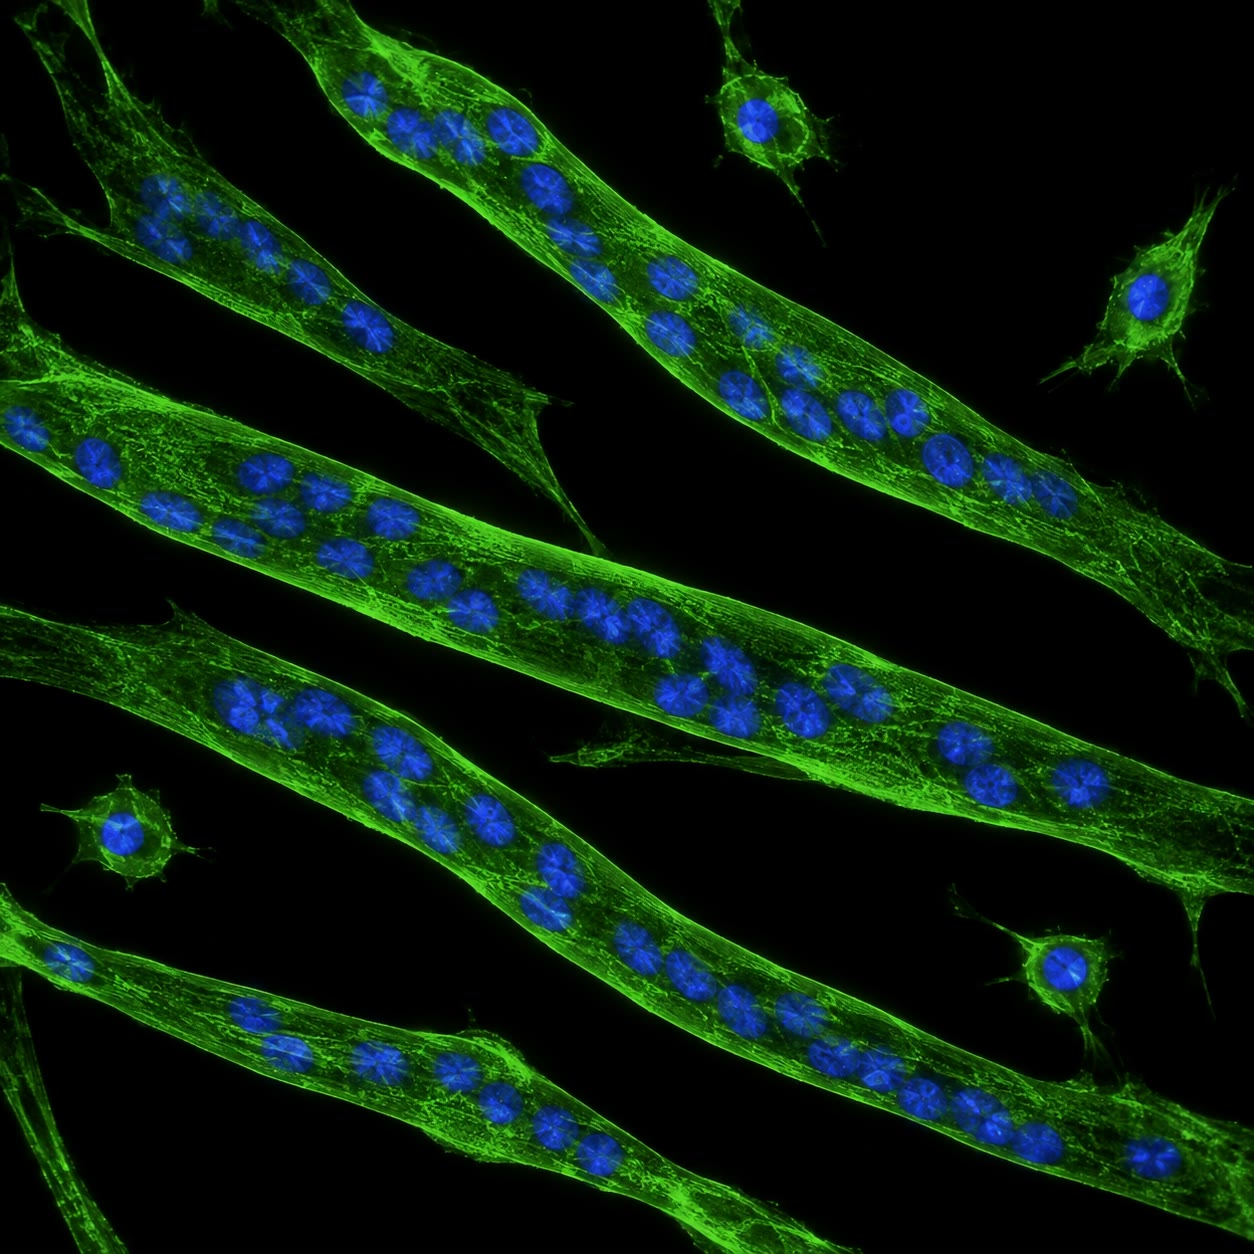
\includegraphics[width=0.44\linewidth]{images/book4/ai/b4-12-myotubes.jpg}\hspace{0.04\linewidth}
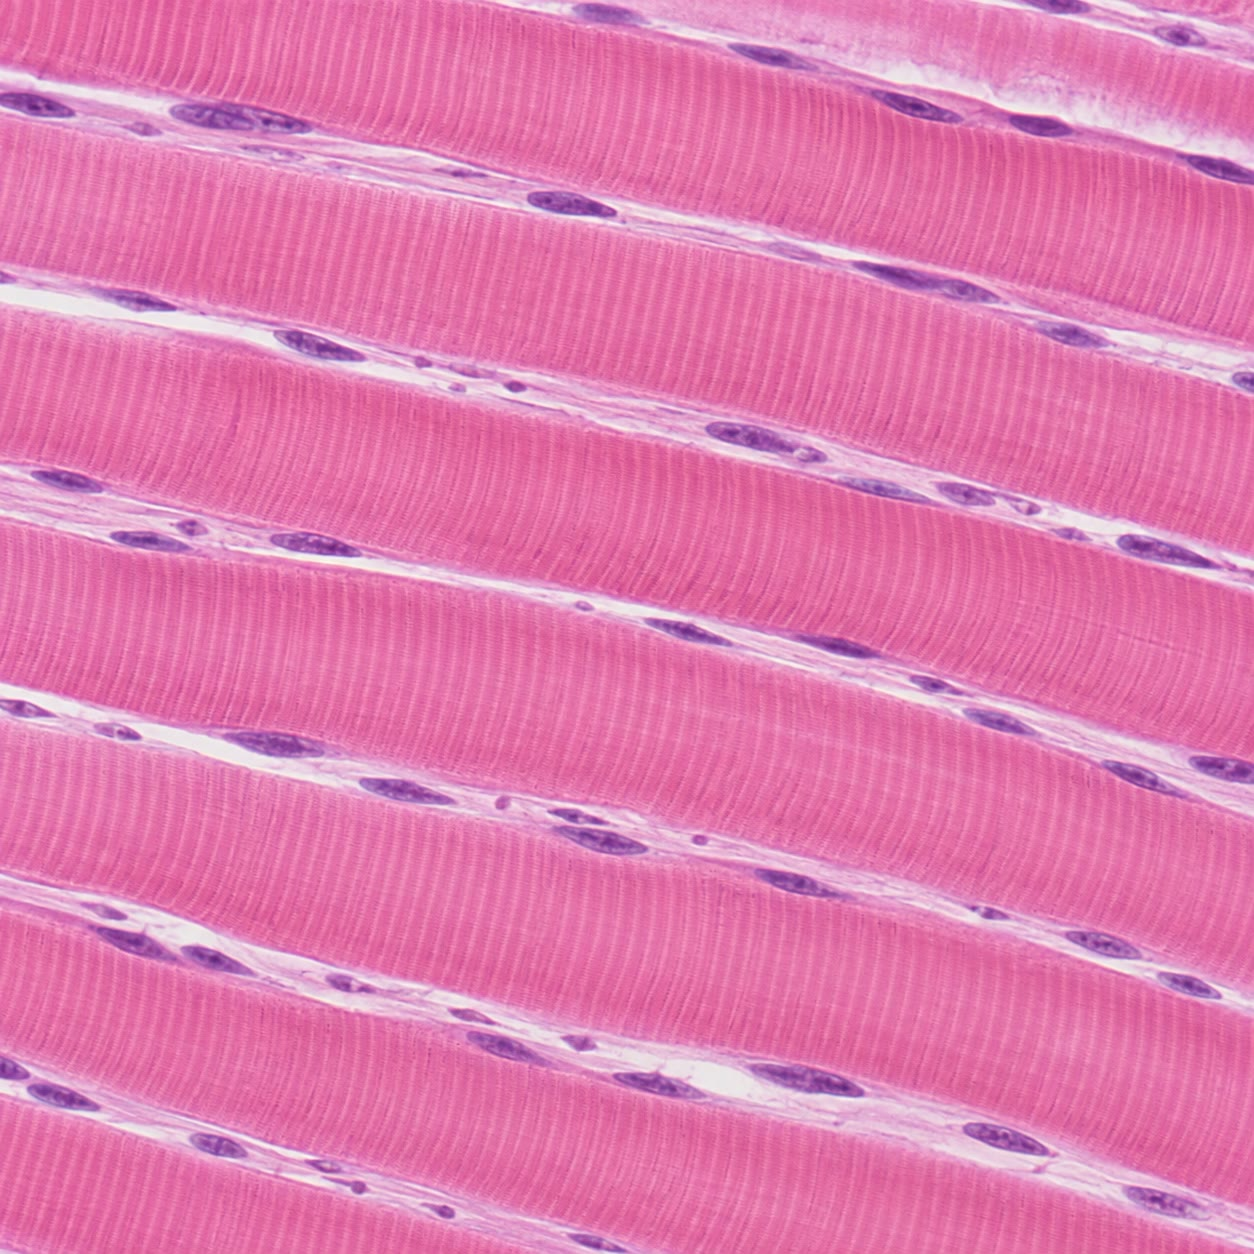
\includegraphics[width=0.44\linewidth]{images/book4/ai/b4-12-muscle-fibres.jpg}

{\small على اليمين: أنابيب عضلية في مزرعة، كل منها خلية مندمجة فيها صف
من النوى، وبجانبها أرومات عضلية مفردة لم تندمج بعد. وعلى اليسار:
ليفات ناضجة في منظر طولي، وتخططاتها العرضية هي
القسيمات العضلية المتكررة ونواها مدفوعة إلى الحافة.}
\end{omfigure}

\begin{proposition}[MyoD: مفتاح رئيس]\label{prop:b2:cell-differentiation:myod}
\index{منظّم رئيس!MyoD}
\omterm{def:b2:cell-differentiation:myogenesis}{MyoD} \omterm{prop:b2:cell-differentiation:transcriptional}{عامل استنساخ} من أسرة اللولب--العروة--اللولب. وهو
يرتبط، ثنائيًا مع بروتين شريك كلي الوجود، بتسلسل من ستة أسس
(هو الصندوق E، وهو CANNTG) في المناطق التنظيمية لمورّثات
العضل، ويجنّد إنزيمات فاتحة للصبغين، ويشعل المورّثات
--- ومنها مورّثتا الميوجينين \omterm{def:b2:cell-differentiation:myogenesis}{وMyoD} نفسه، وهكذا
تثبت الحالة. ونشاطه مبوَّب: ففي الأرومات العضلية المنقسمة يحتجز
بروتين مثبط (Id)، تستحثه عوامل النمو، الشريكَ
ويبقي \omterm{def:b2:cell-differentiation:myogenesis}{MyoD} خاملًا؛ وحين تُسحب عوامل النمو يزول Id
ويعمل \omterm{def:b2:cell-differentiation:myogenesis}{MyoD}. ولأن \omterm{def:b2:cell-differentiation:myogenesis}{MyoD} كافٍ لفرض
برنامج العضل على أرومة ليفية أو خلية شحمية أو خلية عصبية، يكون
مصير العضل، بمعنًى ما، بعمق مورّثة واحدة: فصعوبة
صيرورة عضل ليست في معرفة الكيفية، بل في أن يُقال لك أن تفعل.
\end{proposition}
\begin{proof}[شواهد]
نقل دايفيس ووينتراوب ولاسار (1987) نسخة cDNA واحدة،
معزولة من أرومات عضلية، إلى أرومات ليفية مزروعة: فكفّت الأرومات الليفية
عن الانقسام، واندمجت أنابيب عضلية، وصنعت بروتينات العضل.
وسُمّيت المورّثة \omterm{def:b2:cell-differentiation:myogenesis}{MyoD}. ووُجدت أقاربها Myf5 والميوجينين وMRF4
بالتماثل؛ والفأر الذي يفتقر إلى \omterm{def:b2:cell-differentiation:myogenesis}{MyoD} وMyf5 معًا لا أرومات
عضلية له ولا عضل هيكلي البتة، والفأر الذي يفتقر إلى
الميوجينين له أرومات عضلية لا تندمج أبدًا.
\end{proof}

\begin{theorem}[مفتاح يصون نفسه]\label{thm:b2:cell-differentiation:switch}
\index{ثنائية الاستقرار}\index{تغذية راجعة موجبة!مورّثية}
ليكن $m$ مقدار عامل ينشّط مورّثته هو باستجابة
تعاونية (سينية) ويتحلل بمعدل $k$:
\[
\frac{\mathrm{d}m}{\mathrm{d}t} = \frac{a\,m^{2}}{K^{2} + m^{2}} + b - k\,m,
\]
حيث $b$ اصطناع قاعدي صغير. ومن أجل قيم مناسبة للثوابت $a$ و$b$ و$K$ و
$k$ يكون لهذه المعادلة حالتان مستقرتان \emph{اثنتان}، دنيا
قرب $b/k$ وعليا قرب $a/k$، تفصل بينهما عتبة
غير مستقرة: فالخلية \emph{\omterm{thm:b2:cell-differentiation:switch}{ثنائية الاستقرار}}. والإشارة الاستحثاثية
العابرة التي تدفع $m$ فوق العتبة ترسل الخلية إلى
الحالة العليا، حيث تبقى بعد زوال الإشارة؛ ودون
العتبة تعود إلى الحالة الدنيا. وهذه ذاكرة مبنية من
حلقة تغذية راجعة، وهي سبب بقاء الخلية، متى التزمت،
ملتزمةً عبر الانقسامات وفي غياب المستحِث.
\end{theorem}
\begin{proof}
تحقق الحالات المستقرة $k m = a m^{2}/(K^{2} + m^{2}) + b$. و
الطرف الأيمن منحنٍ سيني يرتفع من $b$ إلى $a + b$؛ والأيسر
مستقيم يمر بالمبدأ ميله $k$. ومن أجل $b/k < K$ و$k$ صغير
بما يكفي ليقطع المستقيم الجزء الحاد من المنحني، يتقاطع
المنحنيان ثلاث مرات: عند $m_{\text{الدنيا}} \approx b/k$، وعند
$m_{\text{ح}}$ وسطية، وعند $m_{\text{العليا}} \approx (a +
b)/k$. والاستقرار: فدون $m_{\text{الدنيا}}$ يفوق الاصطناع التحلل و
يرتفع $m$؛ وبين $m_{\text{الدنيا}}$ و$m_{\text{ح}}$ يفوق التحلل
الاصطناع ويهبط $m$؛ وبين $m_{\text{ح}}$ و
$m_{\text{العليا}}$ يفوق الاصطناع التحلل ويتسلق $m$ إلى
$m_{\text{العليا}}$؛ وفوقها يهبط $m$ عائدًا إلى $m_{\text{العليا}}$.
ومن ثم تكون الطرفيتان مستقرتين والوسطى غير مستقرة وهي
العتبة.
\end{proof}

\begin{omfigure}
\begin{tikzpicture}
\begin{axis}[
  width=0.74\linewidth, height=5.8cm,
  axis x line=bottom, axis y line=left,
  xmin=0, xmax=4, ymin=0, ymax=1.3,
  xlabel={مستوى العامل $m$ (نسبيًا)}, ylabel={المعدل},
  xlabel style={font=\small, at={(axis description cs:0.5,-0.12)}, anchor=north},
  ylabel style={font=\small},
  tick label style={font=\small}, xtick={0,1,2,3,4}, ytick={0,0.5,1},
  legend style={font=\scriptsize, at={(0.03,0.97)}, anchor=north west, draw=none},
  clip=false,
]
\addplot[very thick, omDef, domain=0:4, samples=100] {x^2/(1+x^2) + 0.02};
\addlegendentry{الاصطناع: $a m^2/(K^2 + m^2) + b$}
\addplot[very thick, omThm, domain=0:3.2, samples=2] {0.4*x};
\addlegendentry{التحلل: $k m$}
\fill[omDef] (axis cs:0.055,0.022) circle (2pt); \draw[gray] (axis cs:0.08,0.04) -- (axis cs:0.33,0.42); \node[font=\scriptsize, anchor=west] at (axis cs:0.35,0.45) {مطفأ};
\draw[gray, thick] (axis cs:0.41,0.164) circle (2pt); \node[font=\scriptsize, anchor=west] at (axis cs:0.55,0.10) {العتبة};
\fill[omDef] (axis cs:2.1,0.84) circle (2pt); \node[font=\scriptsize, anchor=north] at (axis cs:2.1,0.78) {مشتعل};
\end{axis}
\end{tikzpicture}

{\small مفتاح ثنائي الاستقرار ($a = 1$، و$K = 1$، و$b = 0.02$، و$k = 0.4$).
يتقاطع الاصطناع (السيني) والتحلل (المستقيم) ثلاث مرات: أي
حالتان مستقرتان، مطفأة ومشتعلة، وعتبة غير مستقرة بينهما.
والإشارة التي ترفع $m$ فوق العتبة تلزم الخلية
بالحالة المشتعلة إلزامًا دائمًا.}
\end{omfigure}

\section{الخلية النهائية}

\begin{definition}[الليفة العضلية]\label{def:b2:cell-differentiation:fibre}
\index{قسيم عضلي}\index{لييف عضلي}\index{شبكة هيولية عضلية}\index{نبيب T}
\omterm{def:b2:cell-differentiation:myogenesis}{الليفة العضلية} الهيكلية أسطوانة عرضها \qtyrange{10}{100}{\micro m}
وطولها يبلغ عشرات السنتيمترات، يحدها
\emph{غمد الليفة}، ومئات النوى تحته مباشرة. وداخلها
مملوء \emph{بلييفات عضلية} متوازية، كل منها سلسلة من
\emph{القسيمات العضلية} طولها \qty{2.5}{\micro m}: فبين قرصي Z، تتداخل خيوط
رفيعة من الأكتين (مع التروبوميوزين والتروبونين) مرساة عند
القرصين مع خيوط غليظة من الميوزين ممسوكة في
المركز، ويعطي نميط التداخل التخططات. وحول كل
لييف عضلي تخزن شبكة من \emph{الشبكة الهيولية العضلية} الكالسيوم؛
و\emph{النبيبات المستعرضة}، وهي انغماد لغمد الليفة، تجري
بين اللييفات العضلية وتحمل الإشارة الكهربائية من
السطح إلى الداخل. وتحشو المتقدرات الفراغات، ويحوي
السيتوبلازم الغليكوجين وفوسفات الكرياتين، وفي الليفات الحمر،
الميوغلوبين. والخلية مبنية لشيء واحد --- أن تقصر عند الأمر
--- وآلية ذلك الأمر هي
\cref{ch:b2:muscle-movement}.
\end{definition}

\begin{omfigure}
\begin{tikzpicture}[every node/.style={font=\scriptsize}]
  % a stretch of myofibril with two sarcomeres
  \foreach \s in {0,4.4} {
    \begin{scope}[xshift=\s cm]
      \draw[very thick, omThm] (0,-1.1) -- (0,1.1);
      \foreach \y in {-0.9,-0.5,-0.1,0.3,0.7} { \draw[thick, omDef] (0,\y) -- (1.6,\y); \draw[thick, omDef] (4.4,\y) -- (2.8,\y); }
      \foreach \y in {-0.7,-0.3,0.1,0.5,0.9} { \draw[line width=3pt, omExo!80!black] (1.0,\y) -- (3.4,\y); }
      \draw[gray] (2.2,-1.1) -- (2.2,1.1);
    \end{scope}
  }
  \draw[very thick, omThm] (8.8,-1.1) -- (8.8,1.1);
  \node[omThm, below] at (0,-1.15) {قرص Z};
  \node[omThm, below] at (4.4,-1.15) {قرص Z};
  \node[omThm, below] at (8.8,-1.15) {قرص Z};
  \node[omDef, above] at (0.8,1.15) {خيوط رفيعة (أكتين)};
  \node[omExo!80!black, above] at (6.6,1.15) {خيوط غليظة (ميوزين)};
  \node[gray, below] at (2.2,-1.15) {الخط M};
  \draw[<->] (0,1.9) -- (4.4,1.9); \node[above] at (2.2,1.9) {قسيم عضلي واحد، \qty{2.5}{\micro m}};
  \draw[<->] (5.4,-1.6) -- (7.8,-1.6); \node[below] at (6.6,-1.6) {النطاق A (القاتم)};
  \draw[<->] (7.8,-1.6) -- (9.8,-1.6); \node[below] at (8.8,-1.6) {النطاق I (الفاتح)};
\end{tikzpicture}

{\small قسيمان عضليان من \omterm{def:b2:cell-differentiation:fibre}{لييف عضلي}: تتداخل خيوط الأكتين الرفيعة المرساة
عند قرصي Z مع خيوط الميوزين الغليظة المتمركزة على
الخط M. ويعطي التداخل النطاق A القاتم والنطاق I الفاتح في
التخططات.}
\end{omfigure}

\begin{proposition}[أصناف الليفات]\label{prop:b2:cell-differentiation:types}
\index{أصناف الليفات العضلية}
العضلة خليط من أصناف الليفات، تضبطه جزئيًا سلالة الأرومات
العضلية وجزئيًا العصب الذي يعصّب الليفة.
فالليفات \emph{البطيئة الأكسدية} (الصنف I) لها ميوزين بطيء، ومتقدرات
وشعيرات كثيرة، وميوغلوبين --- فهي حمراء لا تكل،
مبنية للقوام والتحمل. والليفات \emph{السريعة التحللية السكرية} (الصنف IIx)
لها ميوزين سريع، ومتقدرات قليلة، وغليكوجين كثير ---
فهي بيضاء قوية تُنهك في دقيقة. والليفات \emph{السريعة الأكسدية}
(الصنف IIa) بينهما. وربلة العدّاء أكثرها ليفات
سريعة، وربلة عدّاء الماراثون أكثرها بطيئة، والنسب
موروثة؛ لكن الصنف ليس ثابتًا: فتعصيب عضلة سريعة
بعصب بطيء، أو أشهر من تدريب التحمل، يحول
الليفات نحو الصنف البطيء، لأن نميط نبضات العصب
يبدّل مورّثات أشكال الميوزين ومورّثات تكوّن المتقدرات.
فالخلية المتمايزة تحفظ هويتها ليفةً
عضلية ومع ذلك تنقّح برنامجها استجابةً للاستعمال.
\end{proposition}

\begin{example}[النمو والإصلاح]\label{ex:b2:cell-differentiation:satellite}
تنمو العضلة عند البالغ لا بإضافة ليفات بل بتكبيرها:
فالتدريب يضيف لييفات عضلية إلى كل ليفة، وتندمج فيها \emph{الخلايا
التابعة} لتوفّر النوى الزائدة التي يحتاجها سيتوبلازم أكبر.
وبعد الإصابة تنقسم الخلايا نفسها، وتعيد التعبير عن \omterm{def:b2:cell-differentiation:myogenesis}{MyoD}، وتندمج
وتعيد بناء المقطع المتضرر في غضون أسابيع --- أي البرنامج
الجنيني يُدار من جديد في البالغ. وفي الحثل العضلي تفتقر الليفات
إلى الديستروفين، وهو بروتين يربط اللييفات العضلية
بالغشاء، فتتمزق أثناء التقلص؛ وتصلحها الخلايا التابعة
مرة بعد مرة حتى ينفد المخزون، بعد سنوات، ويحل
النسيج الليفي محل العضلة.
\end{example}

\begin{omfigure}
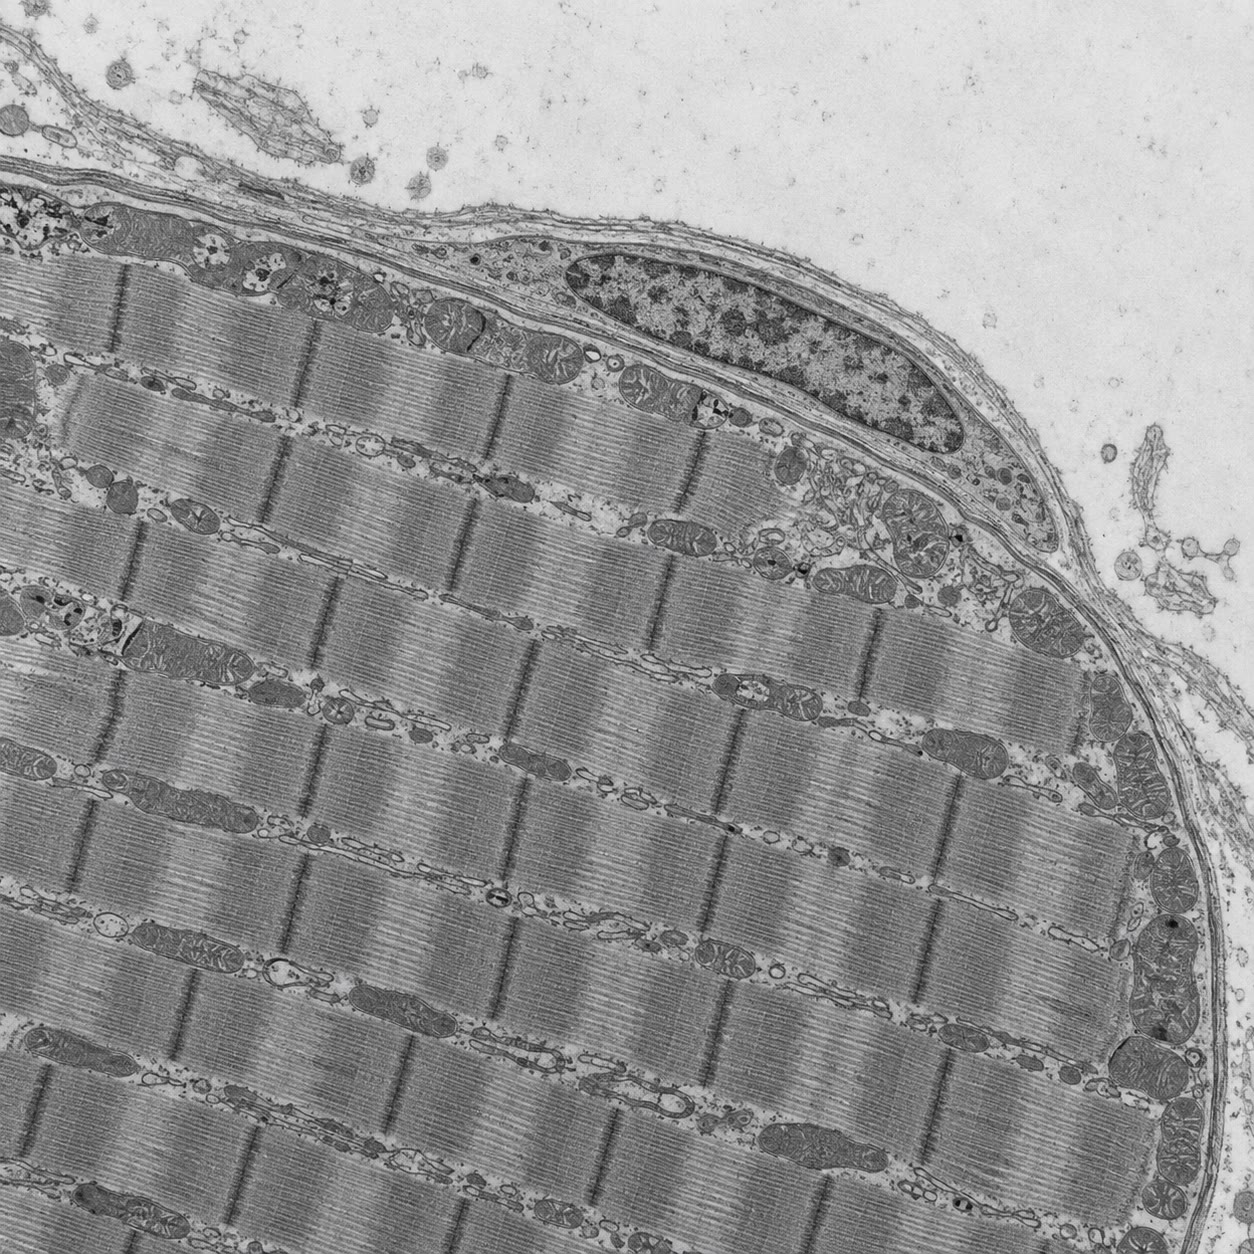
\includegraphics[width=0.42\linewidth]{images/book4/ai/b4-12-satellite-cell-tem.jpg}

{\small خلية تابعة تحت المجهر الإلكتروني: خلية صغيرة
وحيدة النواة محشورة بين غشاء \omterm{def:b2:cell-differentiation:myogenesis}{ليفة عضلية} و
صفيحتها القاعدية --- أي احتياطي الليفة من الأرومات العضلية.}
\end{omfigure}

\section{تمارين}

\begin{exercise}[$\star$]\label{exo:b2:cell-differentiation:1}
عرّف \omterm{def:b2:cell-differentiation:differentiation}{التمايز} \omterm{def:b2:cell-differentiation:differentiation}{والتحدد} والقدرة، وضع اللاقحة
وخلية من \omterm{def:b2:mammal-reproduction:implantation}{الكتلة الخلوية الداخلية} وخلية تابعة \omterm{def:b2:cell-differentiation:myogenesis}{وليفة عضلية}
على سلم القدرة.
\end{exercise}

\begin{exercise}[$\star$]\label{exo:b2:cell-differentiation:2}
اذكر خطوات تكوّن العضل من خلية القُطَيعة إلى \omterm{def:b2:cell-differentiation:myogenesis}{الليفة العضلية}، مع
\omterm{prop:b2:cell-differentiation:transcriptional}{عامل الاستنساخ} المعبَّر عنه في كل خطوة.
\end{exercise}

\begin{exercise}[$\star$]\label{exo:b2:cell-differentiation:3}
ماذا بيّن نقل النوى عند غوردون، وماذا لم يبيّن؟
\end{exercise}

\begin{exercise}[$\star$]\label{exo:b2:cell-differentiation:4}
سمِّ أجزاء \omterm{def:b2:cell-differentiation:fibre}{القسيم العضلي} وقل أيها يتحرك وأيها لا يتحرك
حين تقصر الليفة.
\end{exercise}

\begin{exercise}[$\star\star$]\label{exo:b2:cell-differentiation:5}
ليفة طولها \qty{20}{cm} قسيماتها العضلية \qty{2.5}{\micro m} ولها
نواة كل \qty{25}{\micro m} من طولها. فكم قسيمًا عضليًا
على التوالي، وكم نواة؟ وكم \omterm{def:b2:cell-differentiation:myogenesis}{أرومة عضلية} اندمجت
لصنعها؟
\end{exercise}

\begin{exercise}[$\star\star$]\label{exo:b2:cell-differentiation:6}
اشرح لماذا لا تندمج الأرومات العضلية ما دام FGF حاضرًا، مستعملًا
المثبط Id، وتنبّأ بما يحدث لأرومات عضلية هُندست
لتصنع Id باستمرار.
\end{exercise}

\begin{exercise}[$\star\star$]\label{exo:b2:cell-differentiation:7}
في نموذج المفتاح مع $a = 1$، و$K = 1$، و$b = 0.02$، و$k = 0.4$،
تحقق بالتعويض من أن $m = 2.1$ قريب من حالة مستقرة،
وأوجد الحالة المستقرة الدنيا تقريبًا، وقل ماذا يحدث
لخلية رُفع $m$ فيها إلى $1$ برهةً ثم تُركت وشأنها.
\end{exercise}

\begin{exercise}[$\star\star$]\label{exo:b2:cell-differentiation:8}
في النموذج نفسه يُرفع $k$ إلى $0.6$ (فيتحلل العامل
أسرع). بيّن بيانيًا أو عدديًا أن الحالة العليا
تزول. وبماذا يتنبأ هذا في خلية زُعزع فيها استقرار \omterm{def:b2:cell-differentiation:myogenesis}{MyoD}؟
\end{exercise}

\begin{exercise}[$\star\star$]\label{exo:b2:cell-differentiation:9}
تنبّأ \omterm{def:b2:meiosis-heredity:vocabulary}{بالنمط الظاهري} لفأر يفتقر إلى (أ) \omterm{def:b2:cell-differentiation:myogenesis}{MyoD} وMyf5 معًا،
(ب) الميوجينين وحده، (ج) \omterm{def:b2:cell-differentiation:myogenesis}{MyoD} وحده. ولماذا يكون (ج) شبه سوي؟
\end{exercise}

\begin{exercise}[$\star\star\star$]\label{exo:b2:cell-differentiation:10}
أرومة ليفية مُنقَّلة بالمورّثة \omterm{def:b2:cell-differentiation:myogenesis}{MyoD} تصير أنبوبًا عضليًا؛ وخلية كبدية
مُنقَّلة بالمورّثة نفسها لا تصير. اقترح تفسيرًا يشمل الصبغين
\omterm{def:b2:vertebrate-development:induction}{والأهلية}، وتجربةً لاختباره.
\end{exercise}

\begin{exercise}[$\star\star\star$]\label{exo:b2:cell-differentiation:11}
يحوّل تدريب التحمل الليفات السريعة نحو البطيئة دون
تغيير مورثومها. اشرح بدلالة التعبير المورّثي كيف يستطيع
نميط إطلاق العصب فعل ذلك، ولماذا تبقى الليفات مع ذلك
عضلًا هيكليًا ولا تصير، مثلًا، غضروفًا.
\end{exercise}

\begin{exercise}[$\star\star\star$]\label{exo:b2:cell-differentiation:12}
«الخلية المتمايزة تتذكر ما هي بدارة لا
\omterm{def:b2:genome-diversification:mutation}{بطفرة}.» ناقش، بالمفتاح الثنائي الاستقرار، والصبغين، و
كون إعادتي الضبط عند غوردون وياماناكا ممكنتين لكن
قليلتي الكفاءة.
\end{exercise}

\section{مسألة: عضلة تُبنى وتُعاد بناؤها}

\begin{problem}[{مسألة نهاية الأسبوع --- متابعة عضلة من القُطَيعة إلى
الليفة وعبر الإصابة: أعداد الأرومات العضلية والاندماجات والنوى،
وتحليل المفتاح الثنائي الاستقرار، وتوقيت إصلاح، وقياس التدريب،
وتنتهي إلى عدد نوى الليفة وعتبة المفتاح
وزمن الإصلاح}]
\label{pb:b2:cell-differentiation:1}
لعضلة فخذ بالغ \num{500000} ليفة، طول كل منها
\qty{20}{cm} وقطرها \qty{60}{\micro m}، وفيها
نواة لكل \qty{25}{\micro m} من الطول؛ والقسيمات العضلية
\qty{2.5}{\micro m}. وتنقسم الأرومات العضلية الجنينية كل \qty{12}{h}
ما دام FGF حاضرًا. ونموذج المفتاح: $a = 1$، و$K = 1$، و$b = 0.02$، و$k
= 0.4$. وبعد إصابة تتلف \qty{10}{\%} من طول كل ليفة،
تنقسم الخلايا التابعة في المقطع المصاب (وعددها \num{4} في
المليمتر من الليفة) كل \qty{18}{h} زمنًا ثم تندمج.

\medskip
\noindent\textbf{الجزء الأول --- الليفة.}
\begin{enumerate}
  \item احسب عدد القسيمات العضلية على التوالي في ليفة واحدة و
        عدد النوى.
  \item كم \omterm{def:b2:cell-differentiation:myogenesis}{أرومة عضلية} اندمجت لصنع ليفة واحدة؟ والعضلة كلها؟
  \item احسب حجم ليفة واحدة وحجم العضلة (باللترات).
  \item قدّر الحجم السيتوبلازمي الذي تخدمه نواة واحدة، و
        قارنه بخلية عادية حجمها \qty{2000}{\micro m^3}.
  \item لماذا تقع النوى عند محيط الليفة الناضجة؟
  \item انحدرت أرومات العضلة العضلية من \num{2000} خلية
        قُطَيعة. فكم مضاعفة لزمتها، وكم يومًا،
        لتبلغ عدد السؤال 2؟
\end{enumerate}

\medskip
\noindent\textbf{الجزء الثاني --- المفتاح.}
\begin{enumerate}[resume]
  \item اكتب شرط الحالة المستقرة وبيّن أن $m \approx
        0.055$ يحققه.
  \item بيّن أن $m \approx 2.1$ يحققه.
  \item بيّن أن ثمة حلًا ثالثًا قرب $m = 0.41$، و
        اشرح من إشارتي $\mathrm{d}m/\mathrm{d}t$ على جانبيه
        أنه غير مستقر.
  \item نبضة من مستحِث ترفع $m$ إلى $0.6$؛ وأخرى إلى $0.3$.
        فما مصير كل خلية؟
  \item يُرفع الاصطناع القاعدي $b$ إلى $0.4$ \omterm{def:b2:genome-diversification:mutation}{بطفرة}.
        بيّن أن الحالة الدنيا تزول. فماذا تفعل الخلية؟
  \item اشرح كيف يفسر هذا النموذج بقاء الالتزام عبر
        الانقسام الخلوي، وما الذي يجب أن يصدق على $m$ عند كل انقسام.
\end{enumerate}

\medskip
\noindent\textbf{الجزء الثالث --- الإصلاح.}
\begin{enumerate}[resume]
  \item كم خلية تابعة تحمل ليفة واحدة، وكم نواة
        يجب تعويضها بعد الإصابة؟
  \item كم مضاعفة يجب أن تمر بها الخلايا التابعة
        لتوفيرها، وكم يستغرق ذلك؟
  \item قارن ذلك بالأسبوعين إلى الثلاثة المرصودة للإصلاح، و
        قل ماذا يشمل الزمن أيضًا.
  \item لماذا يجب أن تعيد الخلايا التابعة التعبير عن \omterm{def:b2:cell-differentiation:myogenesis}{MyoD} قبل الاندماج،
        ولماذا يجب أن تكف عن الانقسام أولًا؟
  \item كل جولة إصلاح تستهلك بعض الخلايا التابعة. فإذا هبط
        المخزون \qty{5}{\%} في كل إصابة، فكم إصابة
        قبل أن ينتصف؟
  \item كم خلية تابعة في الليفة تبقى بعد عشرين إصابة
        كهذه؟
  \item اشرح لماذا يحل النسيج الليفي بعد سنوات محل عضلة
        حثلية تتمزق ليفاتها عند كل تقلص.
\end{enumerate}

\medskip
\noindent\textbf{الجزء الرابع --- التدريب.}
\begin{enumerate}[resume]
  \item يثخّن التدريب كل ليفة إلى \qty{80}{\micro m}. فبأي
        عامل ينمو حجم الليفة، وكم نواة زائدة
        يجب أن توفرها الخلايا التابعة إذا حُفظت نسبة
        السؤال 4؟
  \item احسب حجم العضلة الجديد.
  \item يحول تدريب التحمل \qty{30}{\%} من الليفات السريعة
        إلى بطيئة. فما الذي تغير في تلك الليفات وما الذي لم يتغير؟
  \item اشرح لماذا تكبر عضلة البالغ بنمو الليفات
        لا بإضافة ليفات، مستعملًا كون الليفات
        لا تنقسم.
  \item دواء يسد اندماج الخلايا التابعة. تنبّأ
        باستجابة العضلة للتدريب وللإصابة.
  \item اذكر النتيجة: عدد نوى الليفة، وعتبة
        المفتاح، وزمن توفير الخلايا التابعة لنوى إصلاح.
\end{enumerate}
\end{problem}
